\documentclass{beamer}

\usetheme{McMaster}
\usepackage{math}

%===Specific for this talk===%
\usepackage{algorithm,algorithmicx,algpseudocode}
\newtheorem{proposition}{Proposition}
\DeclareMathOperator{\Span}{span}
\DeclareMathOperator*{\argmin}{argmin}
\DeclareMathOperator{\adj}{adj}
\usepackage{tikz, pgfplots}
\usetikzlibrary{decorations.pathreplacing,positioning,calc,intersections,3d,shapes.geometric,shapes,chains,math,fit,backgrounds}

\title{Nonlinear Preconditioning for the Phase-Field Fracture Model}
\author{Conor McCoid}
\institute{McMaster University}
\date{August 1st, 2025}

\begin{document}

\maketitle

\section{Phase-field Fractures}

\begin{frame}
\frametitle{Phase-field energy}

Energy in the phase-field model combines elastic potential energy with energy related to the size and shape of any fractures in the material:
\begin{align*}
E(u,v) = & \frac{1}{2} \int_\Omega \left ( (1-v)^2 + k_\ell \right ) \sigma_0(u) \cdot \epsilon(u) d\Omega \\
		& + \frac{G_c}{c_w} \int_\Omega \frac{v^2}{\ell} + \ell \lvert \nabla v \rvert^2 d\Omega,
\end{align*}
where $\sigma_0$ is the stress tensor, $\epsilon$ is the strain tensor, $\ell$ is a regularization parameter, $k_\ell$, $G_c$ and $c_w$ are constants, $u \in W^{1,2}(\Omega)$ is the displacement and $v \in W^{1,2}(\Omega; [0,1])$ is the auxiliary variable representing damage on the material.

\end{frame}

\begin{frame}
\frametitle{Minimizing the energy}

A solution to the model minimizes this energy:
\begin{equation*}
\hat{u}, \hat{v} = \argmin_{u,v} E(u,v) - f,
\end{equation*}
where $f$ represents external work on the system causing stress, incremented in quasi-static steps to mimic gradually increasing stress.
Irreversibility conditions are placed on $\hat{v}$, so that damage isn't `repaired'.

This minimization problem is non-convex.

\end{frame}

\begin{frame}
\frametitle{Alternate Minimization (AltMin)}

\textbf{But} these two problems \textit{are} convex:
\begin{align*}
	u_{k+1} = & \argmin_u E(u, v_k) - f, \\ v_{k+1} = & \argmin_v E(u_{k+1}, v) - f.
\end{align*}

This algorithm, AltMin, then has guaranteed convergence to at least a local minimum of $E(u,v)$.

\end{frame}

\begin{frame}
\frametitle{AltMin slow-downs}

In practice, AltMin takes a long time at critical moments of the model, usually when cracks begin to propagate.
\href{MOV_CTFM_propagation.mp4}{\textcolor{blue}{(animation)}}

\begin{figure}
	\centering
	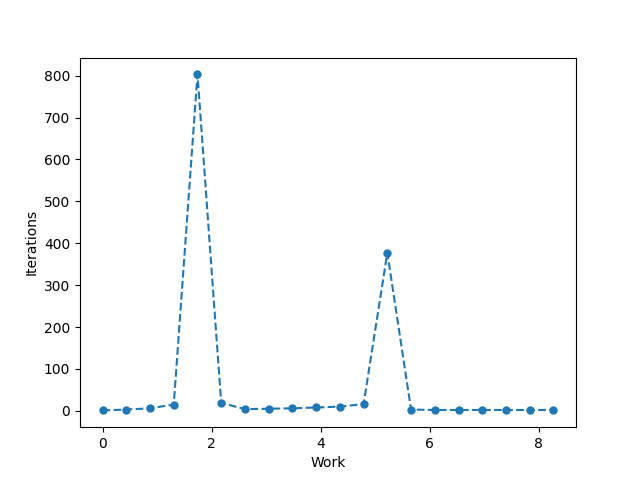
\includegraphics[width=0.8\textwidth]{PLOT_CTFM_its.png}
\end{figure}


\end{frame}

\section{Accelerating with Newton's method}

\begin{frame}
\frametitle{Speed-ups in AltMin}

The proposed solution to AltMin slow-downs is to accelerate the algorithm with Newton's method.
Since AltMin is equivalent to multiplicative Schwarz, the result is MSPIN: Multiplicative Schwarz Preconditioning Inexact Newton.

This approach has shown some effectiveness \footnote{A. Kopanicakova, H. Kothari, R. Krause, \textbf{Nonlinear field-split preconditioners for solving monolithic phase-field models of brittle fracture}, Comput. Methods Appl. Mech. Engrg. 403 (2023)}.
However, traditional MSPIN cannot guarantee convergence like AltMin can.
This could lead to robustness issues if we're not careful.
\end{frame}

\begin{frame}
\frametitle{AltMin as fixed point iteration}

\begin{equation*}
	(u_{k+1}, v_{k+1}) = g(u_k,v_k),
\end{equation*}
where $g(x,y)$ represents the two steps of AltMin:
\begin{equation*}
	g(x,y) = \begin{pmatrix} \argmin\limits_u E(u, y) \\ \argmin\limits_v E(\argmin\limits_u E(u,y), v) \end{pmatrix}.
\end{equation*}

We seek the fixed point of $g(x,y)$:
\begin{equation*}
	g(\hat{u}, \hat{v}) = (\hat{u}, \hat{v}).
\end{equation*}

\end{frame}

\begin{frame}
\frametitle{AltMin + INK}

To accelerate AltMin, consider the function with root at the fixed point:
\begin{equation*}
	f(x,y) = g(x,y) - (x,y).
\end{equation*}
The Jacobian of this function is
\begin{equation*}
	J(x,y) = \begin{pmatrix} E_{uu} \\ E_{vu} & E_{vv} \end{pmatrix}^{-1} \begin{pmatrix} E_{uu} & E_{uv} \\ E_{vu} & E_{vv} \end{pmatrix}
\end{equation*}

We can then approximately solve
\begin{equation*}
	J(x,y) p = -f(x,y),
\end{equation*}
with an inexact Newton-Krylov method,
then setting $(u_{k+1}, v_{k+1}) = (u_k, v_k) + p$.

\end{frame}

\begin{frame}
\frametitle{The FP/N plane}

We now have two options for iterations from the point $(x,y)$:
$g(x,y)$ (AltMin) and $(x,y) + p$ (MSPIN).

These three points all line within a 2D plane where any subsequent iteration based on these methods could land.
We can then restrict any analysis to this plane.

		\begin{figure}
			\begin{tikzpicture}
				\draw[red, thick] (0,0) circle (50pt);
				\filldraw[blue] (-50pt,0) circle (3pt) node[right] {$(x,y)$};
				\filldraw[black] (-30pt,20pt) circle (3pt) node[right] {$g(x,y)$};
				\draw[green, thick, ->] (-50pt,0) -- (-20pt,-10pt) node[right] {$-p$};
				\draw[green, thick, ->] (-50pt,0) -- (-80pt,10pt) node[left] {$p$};
			\end{tikzpicture}
		\end{figure}
\end{frame}

\begin{frame}
\frametitle{Davidenko-Branin trick}

The guaranteed convergence of AltMin suggests using the Davidenko-Branin trick \footnote{R.P. Brent, \textbf{On the Davidenko-Branin method for solving simultaneous nonlinear equations}, IBM J. of R\&D, 16(4):434-436 (1972)}: 
\begin{equation*}
	p = \frac{ \adj J}{\abs{ \det J}} f(x,y)
\end{equation*}
essentially introducing a minus sign if $f(x,y)$ is on the `wrong' side of the true solution.

We can `cheat' and determine whether or not to introduce the sign change by seeing if $p$ or $-p$ points more towards $g(x,y)$.
In the picture below, we would drop $p$ in favour of $-p$.

\begin{figure}
	\begin{tikzpicture}
				\filldraw[blue] (-50pt,0) circle (3pt) node[right] {$(x,y)$};
				\filldraw[black] (-30pt,20pt) circle (3pt) node[right] {$g(x,y)$};
				\draw[green, thick, ->] (-50pt,0) -- (-20pt,-10pt) node[right] {$-p$};
				\draw[green, thick, ->] (-50pt,0) -- (-80pt,10pt) node[left] {$p$};
	\end{tikzpicture}
\end{figure}

\end{frame}

\begin{frame}
\frametitle{Trust region}

\begin{columns}
	\begin{column}{0.5\textwidth}
		Since AltMin is convergent, $g(x,y)$ lies closer to the solution than $(x,y)$.
		\\
		\vspace{1em}
		In the example here, the Newton-Davidenko-Branin step lies closer to the fixed point step than to the current iterate, suggesting we can accept it.
	\end{column}
	\begin{column}{0.5\textwidth}
		\begin{figure}
			\begin{tikzpicture}
				\filldraw[blue] (-50pt,0) circle (3pt) node[right] {$(x,y)$};
				\filldraw[black] (0,0) circle (3pt) node[right] {$g(x,y)$};
				\draw[blue, dashed] (-25pt, -50pt) -- (-25pt, 50pt);
				\draw[green, thick, ->] (-50pt,0) -- (-20pt,-40pt) node[right] {$-p$};
			\end{tikzpicture}
		\end{figure}
	\end{column}
\end{columns}

\end{frame}

\begin{frame}
\frametitle{Line search}

\begin{columns}
	\begin{column}{0.5\textwidth}
		The fixed point step must have a reasonable step size, unlike Newton which may leap a great distance away.
		But the Newton direction may be preferable.
		\\
		\vspace{1em}
		Choose to step in the Newton direction with step size equal to the fixed point length, or some multiple of it.
	\end{column}
	\begin{column}{0.5\textwidth}
		\begin{figure}
			\begin{tikzpicture}
				\filldraw[blue] (-50pt,0) circle (3pt) node[left] {$(x,y)$};
				\filldraw[black] (0,0) circle (3pt) node[right] {$g(x,y)$};
				\draw[black, thick] (-50pt,0) -- (0,0) node[above, midway] {$h$};
				\filldraw[green] (50pt,-30pt) circle (3pt) node[below] {$(x,y) + p$};
				\draw[green, thick, ->] (-50pt,0) -- (0,-15pt) node[right] {$h$};
			\end{tikzpicture}
		\end{figure}
	\end{column}
\end{columns}

\end{frame}

\begin{frame}
\frametitle{Two-step}

\begin{columns}
	\begin{column}{0.5\textwidth}
		Take the fixed point step, then step towards the Newton step, but only part of the way.
		\\
		\vspace{1em}
		We want $\alpha$ to be larger (but at most 1) if the distance between $g(x,y)$ and $(x,y) + p$ is smaller, as we can have more confidence in the results.
	\end{column}
	\begin{column}{0.5\textwidth}
		\begin{figure}
			\begin{tikzpicture}
				\filldraw[blue] (-50pt,0) circle (3pt) node[left] {$(x,y)$};
				\filldraw[black] (0,0) circle (3pt) node[right] {$g(x,y)$};
				\draw[black, thick] (-50pt,0) -- (0,0) node[above, midway] {$h$};
				\filldraw[green] (50pt,-30pt) circle (3pt) node[below] {$(x,y) + p$};
				\draw[green, thick, ->] (0,0) -- (40pt,-25pt) node[above right] {$\alpha$};
			\end{tikzpicture}
		\end{figure}
	\end{column}
\end{columns}

\end{frame}

\begin{frame}
\frametitle{Comparing methods}

\begin{figure}
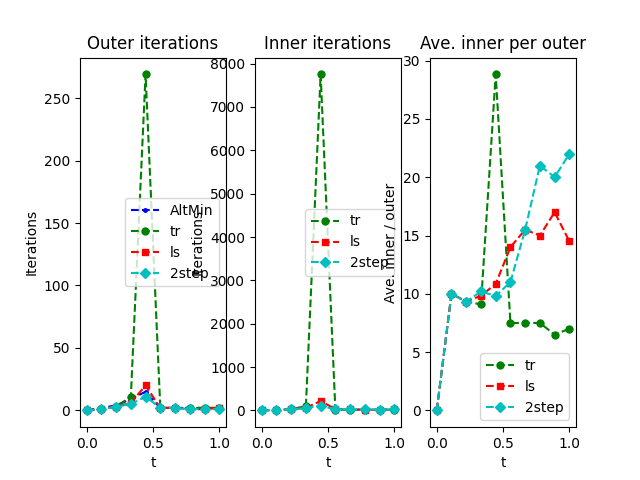
\includegraphics[width=\textwidth]{FIG_GD_its_full.png}
\end{figure}

\end{frame}

\begin{frame}
\frametitle{Comparing methods}

\begin{figure}
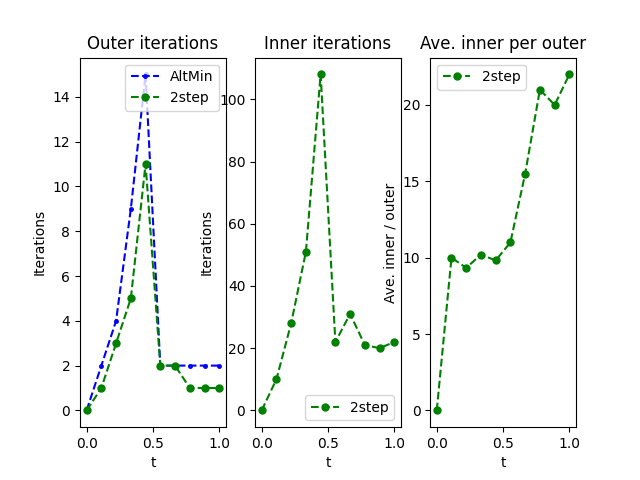
\includegraphics[width=\textwidth]{FIG_GD_its_2step.png}
\end{figure}
\end{frame}

\begin{frame}
\frametitle{Conclusions and future work}

\begin{itemize}
\item We can leverage the guaranteed convergence of AltMin to get more robust MSPIN algorithms
\item We can develop geometric combinations of fixed point and Newton methods
\item More analysis is needed for more sophisticated methods
\end{itemize}

\end{frame}

\end{document}